%===========================================
\chapter{Décomposer le problème}
\index{décomposer le code}
%===========================================

%===================
\section{Motivation}
%===================

	Jusqu'à présent, 
	les problèmes que nous avons abordés étaient relativement petits.
	Nous avons pu les résoudre avec un algorithme d'un seul tenant.
	
	Dans la réalité,
	les problèmes sont plus gros 
	et il devient nécessaire de les décomposer en sous-problèmes.
	On parle d'une \emph{approche modulaire}.
	Les avantages d'une telle décomposition sont multiples.
	\begin{itemize}
	\item
		\textbf{Cela permet de libérer l'esprit.}
		L'esprit humain ne peut pas traiter trop d'informations à la fois
		(\emph{surcharge cognitive}).
		Lorsqu'un sous-problème est résolu,
		on peut se libérer l'esprit et attaquer un autre sous-problème.
	\item
		\textbf{On peut réutiliser ce qui a été fait.}
		Si un même sous-problème apparait plusieurs fois
		dans un problème ou à travers plusieurs problèmes,
		il est plus efficace de le résoudre une fois et
		de réutiliser la solution.
	\item
		\textbf{On accroit la lisibilité.}
		Si, dans un algorithme, 
		on appelle un autre algorithme pour résoudre un sous-problème,
		le lecteur verra un nom d'algorithme qui peut être plus parlant
		que les instructions qui se cachent derrière, même s'il y en a peu.
		Par exemple, \lda{dizaine(nb)} est plus parlant que
		\lda{nb MOD 100 DIV 10} pour calculer les dizaines d'un nombre.
	\end{itemize}

	Parmis les autres avantages, 
	que vous pourrez moins percevoir en début d'apprentissage,
	citons la possibilité de répartir le travail dans une équipe.
	
%===================
\section{Exemple}
%===================

	Illustrons l’approche modulaire sur 
	le calcul du maximum de 3 nombres.

	\begin{center}
	\flowalgoddd{a (réel)}{b (réel)}{c (réel)}{max3}{réel}
	\end{center}
	
	Commençons par écrire la solution du problème plus simple~:~
	le maximum de 2 nombres.

	\begin{minipage}{6cm}
		\flowalgodd{a (réel)}{b (réel)}{max2}{réel}
	\end{minipage}
	\quad
	\begin{minipage}{7cm}
		\begin{LDA}
		\Algo{max2}{\Par{a}{réel}, \Par{b}{réel}}{réel}
			\Decl{max}{réel}
			\If{a > b}
				\Let max \Gets a
			\Else
				\Let max \Gets b
			\EndIf
			\Return max
		\EndAlgo
		\end{LDA}
	\end{minipage}
	
	Pour le maximum de 3 nombres, il existe plusieurs approches.
	Voyons celle-ci~:

	\begin{LDA}
		\Stmt 1) Calculer le maximum des deux premiers nombres, soit \lda{maxab}
		\Stmt 2) Calculer le maximum de \lda{maxab} et du troisième nombre, ce qui donne le résultat.
	\end{LDA}

	Qu'on peut illustrer ainsi :
	
	\begin{center}
	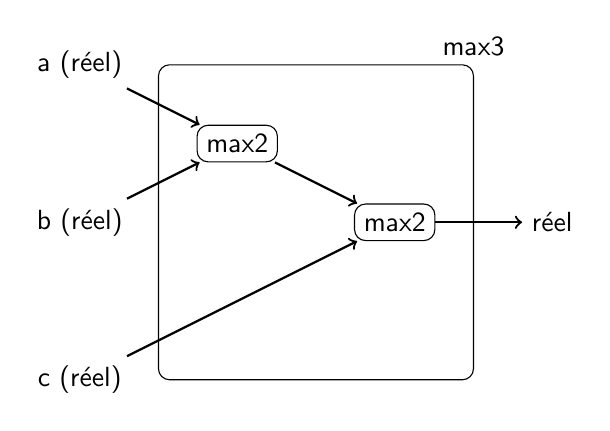
\begin{tikzpicture}[auto]
		\sffamily
		\node (a) at (0,4) {a (réel)};
		\node (b) at (0,2) {b (réel)};
		\node (c) at (0,0) {c (réel)};
		\node[draw,rounded corners] (max2a) at (2,3) {max2};
		\node[draw,rounded corners] (max2b) at (4,2) {max2};
		\node (r) at (6,2) {réel};
		\draw[rounded corners] (1,0) rectangle (5,4) node[above] {max3};
		\draw[->,thick] (a) to (max2a);
		\draw[->,thick] (b) to (max2a);
		\draw[->,thick] (c) to (max2b);
		\draw[->,thick] (max2a) to (max2b);
		\draw[->,thick] (max2b) to (r);
	\end{tikzpicture}	
	\end{center}
	
	Sur base de cette idée, comment faire concrètement
	pour introduire le calcul du maximum de 2 nombres 
	dans l’algorithme calculant le maximum de 3 nombres~? 
	Une solution consiste à «~copier-coller~» 
	les lignes de \lda{max2}
	dans \lda{max3},
	en adaptant son contenu au contexte~:~
	\lda{maxab} est calculé 
	et ré-utilisé dans un calcul ultérieur. 
	Ceci donnerait~:

	\begin{LDA}
	\Algo{max3}{\Par{a}{réel}, \Par{b}{réel}, \Par{c}{réel}}{réel}
		\Decl{maxab, max}{réels}
		\If{a > b}
			\Let maxab \Gets a
		\Else
			\Let maxab \Gets b
		\EndIf
		\If{maxab > c}
			\Let max \Gets maxab
		\Else
			\Let max \Gets c
		\EndIf
		\Return max
	\EndAlgo
	\end{LDA}

	Bien que correcte, cette démarche est cependant déconseillée 
	et peut s’avérer fastidieuse, dangereuse et contre-productive.
	\begin{itemize}
	\item
		Imaginons qu’il eût fallu de cette façon «~mixer~» deux
		algorithmes d’une cinquantaine de lignes chacun. 
		Le résultat serait un algorithme d’une centaine de lignes 
		qui perdrait en lisibilité et clarté. 
	\item
		De plus, l’opération effectuée n’est pas sans risques~:~
		que se passerait-il si les deux algorithmes 
		contiennent chacun une variable nommée de manière identique~? 
		Cette «~transplantation~» demande donc 
		la vérification de toutes les variables utilisées, 
		la réécriture des lignes de déclarations de variables 
		de façon à y inclure celles du module «~greffé~», etc.
	\end{itemize}
	
	Imaginons, par exemple, que l’on doive calculer le
	maximum de 4 ou même 5 nombres. Le résultat serait un code long et
	à l’allure répétitive. Une erreur serait vite arrivée et
	serait difficile à détecter.
	
	Le mieux,
	est d'utiliser (d'appeler) l'algorithme \lda{max2}
	dans \lda{max3}.

	\begin{LDA}
	\Algo{max3}{\Par{a}{réel}, \Par{b}{réel}, \Par{c}{réel}}{réel}
		\Decl{maxab, max}{réels}
		\Let maxab \Gets max2(a,b)
		\Let max \Gets max2(maxab,c)
		\Return max
	\EndAlgo
	\end{LDA}

	qu'on peut encore simplifier en :
	
	\begin{LDA}
	\Algo{max3}{\Par{a}{réel}, \Par{b}{réel}, \Par{c}{réel}}{réel}
		\Return max2( max2(a,b) ,c)
	\EndAlgo
	\end{LDA}

%===================
\section{Les paramètres}
\index{paramètres}
%=======================

	Jusqu'à présent,
	nous avons considéré que les paramètres d'un algorithme (ou \emph{module}\index{module})
	correspondent à ses données et que le résultat, unique,
	est retourné.

	Il s'agit d'une situation fréquente mais pas obligatoire
	que nous pouvons généraliser.
	En pratique, on peut rencontrer trois sortes de paramètres.

	%==================================
	\subsection{Le paramètre en entrée}
	%==================================

		Le paramètre en \textbf{entrée}
		est ce que nous connaissons déjà.
		Il correspond à une donnée de l'algorithme.
		Une valeur va lui être attribuée en début d'algorithme
		et elle ne sera pas modifiée.
		On pourra faire suivre le nom du paramètre d'une flèche
		vers le bas (\In) pour rappeler son rôle.
		
		Lors de l'appel, on fournit la \textbf{valeur}
		ou, plus généralement une expression
		dont la valeur sera donnée au paramète.

		\textbf{Illustration.} 
		Voici un cas général de paramètre en entrée.
		
		\begin{minipage}{4cm}
			\begin{LDA}
				\LComment {Code appelant}
				\Stmt algo(expr)
				\Empty
			\end{LDA}
		\end{minipage}
		\quad
		\begin{minipage}{8cm}
			\begin{LDA}
				\LComment {Code appelé}
				\Entete{monAlgo}{\Par{par\In}{entier}}{}
				\Stmt \dots
			\end{LDA}
		\end{minipage}
		
		C'est comme si l'algorithme \lda{monAlgo}
		commençait pas l'affectation
		\lda{par \Gets expr}.
		
	%==================================
	\subsection{Le paramètre en sortie}
	%==================================

		Le paramètre en \textbf{sortie}
		correspond à un résultat de l'algorithme.
		Avec la notation que nous utilisons,
		un algorithme ne peut retourner qu'une seule valeur
		ce qui est parfois une contrainte trop forte.
		Les paramètres en sortie vont permettre à l'algorithme
		de fournir plusieurs réponses.
		On fera suivre le nom du paramètre d'une flèche
		vers le haut (\Out) pour rappeler son rôle.
		Un tel paramètre n'aura pas de valeur
		au début de l'algorithme mais s'en verra attribuée une
		par l'algorithme.
		
		Lors de l'appel, on fournit une \textbf{variable}
		qui recevra la valeur finale du paramètre.
		
		\paragraph{Exemple.}
		On peut envisager un algorithme
		qui reçoit une durée exprimée en seconde
		et fournisse trois paramètres en sortie
		correspondant à cette même durée exprimée en heures, minutes et secondes.
		En voici le schéma et la solution :
		\begin{center}
		\flowalgorrr{totalSec (entier)}{versHMS}{H (entier)}{M (entier)}{S (entier)}
		\end{center}
			
		\begin{LDA}
			\Algo{versHMS}{\Par{totalSec\In}{entier}, \Par{H\Out}{entier}, 
						   \Par{M\Out}{entier}, \Par{S\Out}{entier}}{}
				\Let H \Gets totalSec DIV (60*60)
				\Let M \Gets totalSec MOD (60*60) DIV 60				
				\Let S \Gets totalSec MOD 60
			\EndAlgo
		\end{LDA}
		
		Il n'y a donc pas de \lda{\algorithmicreturn}
		puisque les résultats sont en paramètres de sortie et pas comme
		valeur \emph{retournée}.
		Un appel possible pourrait être :

		\begin{LDA}
			\Stmt versHMS(65536, heure, minute, seconde)
		\end{LDA}

		C'est comme si,
		à la fin de l'algorithme \lda{versHMS},
		on avait les assignations suivantes :
		\\\lda{heure \Gets H}, \lda{minute \Gets M} et \lda{seconde \Gets S}.
				
	%==================================
	\subsection{Le paramètre en entrée-sortie}
	%==================================

		Le paramètre en \textbf{entrée-sortie}
		correspond à une situation mixte.
		Il est à la fois une donnée et un résultat de l'algorithme.
		Cela signifie que l'algorithme a pour but de le modifier.
		Un tel paramètre sera suivi d'une double flèche (\In\Out).
		
		Lors de l'appel, on fournit \textbf{une variable}.
		Sa valeur est donnée au paramètre au début de l'algorithme.
		À la fin de l'algorithme, la variable reçoit la valeur du paramètre.
		
		\paragraph{Exemple.}
		On a déjà vu un algorithme qui retourne la valeur absolue d'un nombre.
		On pourrait imaginer une variante qui \textbf{modifie}
		le nombre reçu.
		En voici le schéma et la solution :

		\begin{minipage}{6cm}		
			\begin{center}
			\flowalgov{nb (réel)}{valAboslue}
			\end{center}
		\end{minipage}
		\quad
		\begin{minipage}{6cm}		
			\begin{LDA}
				\Algo{valAbsolue}{\Par{nb\In\Out}{réel}}{}
					\If{nb<0}
						\Let nb \Gets -nb
					\EndIf
				\EndAlgo
			\end{LDA}
		\end{minipage}
		
		Un appel possible pourrait être :

		\begin{LDA}
			\Stmt valAbsolue(température)
		\end{LDA}
	
		C'est comme si, dans \lda{valAbsolue},
		on avait une première ligne pour donner sa valeur au paramètre
		(\lda{nb \Gets température})
		et une dernière ligne pour effectuer l'assignation opposée
		(\lda{nb \Gets température}).
		
%==================================
\section{La valeur de retour}
%==================================
	
	Une valeur de retour est toujours possible,
	mais jamais obligatoire,
	quels que soient les sortes des paramètres.
	Ainsi, on peut imaginer un algorithme
	qui possède un paramètre en sortie \textbf{et}
	qui retourne également une valeur.

	Attention !
	Un algorithme qui ne \textbf{retourne} rien (pas de \Gives)
	n'a pas de valeur ;
	il ne peut pas apparaître dans une expression
	ou être assigné à une variable.

%===================
\section{Résumons}
%===================

	Reprenons tout ce qu'on vient de voir
	avec un exemple d'algorithme qui possède tous les types de paramètres.

	\begin{LDA}
		\Algo{test}{}{}
			\Write f(pE1, pE2, pE3)
		\EndAlgo
		\Empty
		\Algo{f}{\Par{pF1\In}{entier}, \Par{pF2\Out}{entier}, \Par{pF3\In\Out}{entier}}{entier}
			\Let{\color{gray} pF1 \Gets pE1} 
			\Let{\color{gray} pF3 \Gets pE3} 
			\Empty
			\LComment Le code proprement dit de l'algorithme
			\Empty
			\Let{\color{gray} pE2 \Gets pF2} 
			\Let{\color{gray} pE3 \Gets pF3} 
			\Return réponse
		\EndAlgo
	\end{LDA}

	Pour mieux se comprendre,
	il est utile d'introduire un peu de vocabulaire.
	Les paramètres déclarés dans l'entête d'un algorithme
	sont appelés \textbf{paramètres formels}.
	Les paramètres donnés à l'appel de l'algorihtme
	sont appelés \textbf{paramètres effectifs}. 
	
	Les instructions en gris dans l'exemple ne sont pas écrites
	mais c'est comme si elles étaient présentes
	pour initialiser les paramètres formels \In{} et \InOut{}
	en début d'algorithme
	et pour donner des valeurs 
	aux paramètres effectifs \Out{} et \InOut{}
	en fin d'algorithme.
	
	On comprend pourquoi \lda{pE1} peut être une expression quelconque
	mais que \lda{pE2} et \lda{pE3} doivent être des variables,
	puisqu'elle vont recevoir une valeur.
	
	À la fin de l'algorithme, 
	c'est comme si la valeur retournée \emph{remplaçait} l'appel.
	Dans notre exemple, c'est donc cette valeur retournée
	qui sera affichée.

	\begin{TODO}
		Si quelqu'un se sent de faire un schéma 
		plus parlant que ce bla-bla\dots
	\end{TODO}
	
%===================
\section{Exercices}
%===================

	\begin{Exercice}{Tracer des algorithmes}
		Indiquer quels nombres sont successivement affichés 
		lors de l’exécution des algorithmes ex1, ex2, ex3 et ex4.
	
		\begin{LDA}
		\Algo{ex1}{}{}
			\Decl{x, y}{entiers}
			\Stmt addition(3, 4, x)
			\Write x
			\Let x \Gets 3
			\Let y \Gets 5
			\Stmt addition(x, y, y)
			\Write y
		\EndAlgo
		\Empty
		\Algo{addition}{a\In, b\In, c\Out~:~entiers}{}
			\Decl{somme}{entier}
			\Let somme \Gets a + b
			\Let c \Gets somme
		\EndAlgo
		\end{LDA}
	
		\begin{LDA}
		\Algo{ex2}{}{}
			\Decl{a, b}{entiers}
			\Stmt addition(3, 4, a) \Comment voir ci-dessus
			\Write a
			\Let a \Gets 3
			\Let b \Gets 5
			\Stmt addition(b, a, b)
			\Write b
		\EndAlgo
		\end{LDA}
	
		\begin{LDA}
		\Algo{ex3}{}{}
			\Decl{a, b, c}{entiers}
			\Stmt calcul(3, 4, c)
			\Write c
			\Let a \Gets 3
			\Let b \Gets 4
			\Let c \Gets 5
			\Stmt calcul(b, c, a)
			\Write a, b, c
		\EndAlgo
		\Empty
		\Algo{calcul}{a\In, b\In, c\Out~:~entiers}{}
			\Let a \Gets 2 * a
			\Let b \Gets 3 * b
			\Let c \Gets a + b
		\EndAlgo
		\end{LDA}
	
		\begin{LDA}
		\Algo{ex4}{}{}
			\Decl{a, b, c}{entiers}
			\Let a \Gets 3
			\Let b \Gets 4
			\Let c \Gets f(b)
			\Write c
			\Stmt calcul2(a, b, c)
			\Write a, b, c
		\EndAlgo
		\Empty
		\Algo{calcul2}{a\In, b\In, c\Out~:~entiers}{}
			\Let a \Gets f(a)
			\Let c \Gets 3 * b
			\Let c \Gets a + c
		\EndAlgo
		\Empty
		\Algo{f}{a\In~:~entier}{entier}
			\Decl{b}{entier}
			\Let b \Gets 2 * a + 1
			\Return b
		\EndAlgo
		\end{LDA}	
	\end{Exercice}
	
	\begin{Exercice}{Appels de module}
		Parmi les instructions suivantes (où les variables
		\lda{a}, \lda{b} et \lda{c}
		sont des entiers), lesquelles font correctement appel 
		à l'algorithme d’en-tête suivant~?
	
		\begin{LDA}
			\Entete{PGCD}{a\In,b\In~:~entiers}{entier}
		\end{LDA}
	
		\begin{LDA}
		\Stmt [1] a \Gets PGCD(24, 32)
		\Stmt [2] a \Gets PGCD(a, 24)
		\Stmt [3] b \Gets 3 * PGCD(a + b, 2*c) + 120
		\Stmt [4] PGCD(20, 30)
		\Stmt [5] a \Gets PGCD(a, b, c)
		\Stmt [6] a \Gets PGCD(a, b) + PGCD(a, c)
		\Stmt [7] a \Gets PGCD(a, PGCD(a, b))
		\Stmt [8] \K{lire} PGCD(a, b)
		\Stmt [9] \K{afficher} PGCD(a, b)
		\Stmt [10] PGCD(a, b) \Gets c
		\end{LDA}
	\end{Exercice}
	
	\begin{Exercice}{Maximum de 4 nombres}
		Écrivez un algorithme qui calcule le maximum de 4 nombres.
	\end{Exercice}

	\begin{Exercice}{Écart entre 2 durées}
		Étant donné deux durées données chacune par trois
		nombres (heure, minute, seconde),
		écrire un algorithme qui calcule
		le délai écoulé entre ces deux durées en heure(s), minute(s),
		seconde(s) sachant que la deuxième durée donnée 
		est plus petite que la première.
	\end{Exercice}
	
	\begin{Exercice}{Validité d'une date}
		Vous avez déjà écrit un algorithme
		qui vérifie la validité d'une date.
		Revenez-y et voyez comment
		vous pouvez le décomposer
		pour accroitre sa lisibilité
		et créer des modules utiles et réutilisables.
	\end{Exercice}

	\begin{Exercice}{Réussir GEN1}
		Reprenons l'exercice \vref{algo:réussirGEN1}.
		Cette fois-ci on ne veut rien afficher
		mais fournir deux résultats :
		un booléen indiquant si l'étudiant a réussi ou pas
		et un entier indiquant sa cote (qui n'a de sens que s'il a réussi). 
	\end{Exercice}
	
